%% content.tex
%%

%% ===========================         
\chapter{Konzeption}
\label{ch:Konzeption}
%% ===========================

Ein Konzept dient in der Softwarearchitektur der Konstruktion eines abstrakten Systemmodells. Zur Gestaltung werden technische Details weggelassen und stattdessen allgemeingültige Begriffe und ihre Zusammenhänge festgelegt. Weiterhin wird ein Grundverständnis durch Definieren von Strukturen und Konzepten gebildet. Darüber hinaus werden Schnittstellen definiert, die Wechselwirkungen zwischen den Komponenten beschreiben. Weiterhin werden im Zuge der Überlegungen Technologien ausgewählt, die zur Umsetzung der verschiedenen Komponenten verwendet werden.

%% ===========================
\section{Architektur}
\label{ch:Konzeption:architektur}
%% ===========================

Zuerst wird ein erster Überblick über den geplanten Aufbau des Systems gegeben. Abbildung \ref{konzept_architektur} zeigt die Komponenten des Systems und der Umwelt. Der Tomcat mit seinen Webcontainern bildet die Basis des Systems. Wie auf der Abbildung zu sehen sind zwei verschiedene Projekte vorgesehen. Zum einen ein Client-Webprojekt und zum anderen ein Server-Webprojekt. Das Client-Webprojekt soll die Klassen und Methoden zur Umsetzung der Darstellung beinhalten. Die Anwendungslogik sowie die Datenbank sind im Server-Webprojekt vorgesehen. Der Grund für die Aufteilung in zwei verschiedene Webprojekte ist die Anforderung der losen Kopplung zwischen Client und Server. Beide Webprojekte werden in Form von Web-Archive-Dateien in einem Apache-Tomcat-Webserver deployed und können über die entsprechende URL angesprochen werden. Weiterhin soll mithilfe eines selbstgeschriebenen Plugins für den CAS genesisWorld Anwendungsserver die Synchronisation zwischen den Systemen umgesetzt werden. Der Browser, CAS genesisWorld und der MSSQL-Server stellen die Umwelt des Systems dar. Im Folgenden wird auf jede Komponente der Architektur eingegangen.

\begin{figure}[htbp]
\centering
  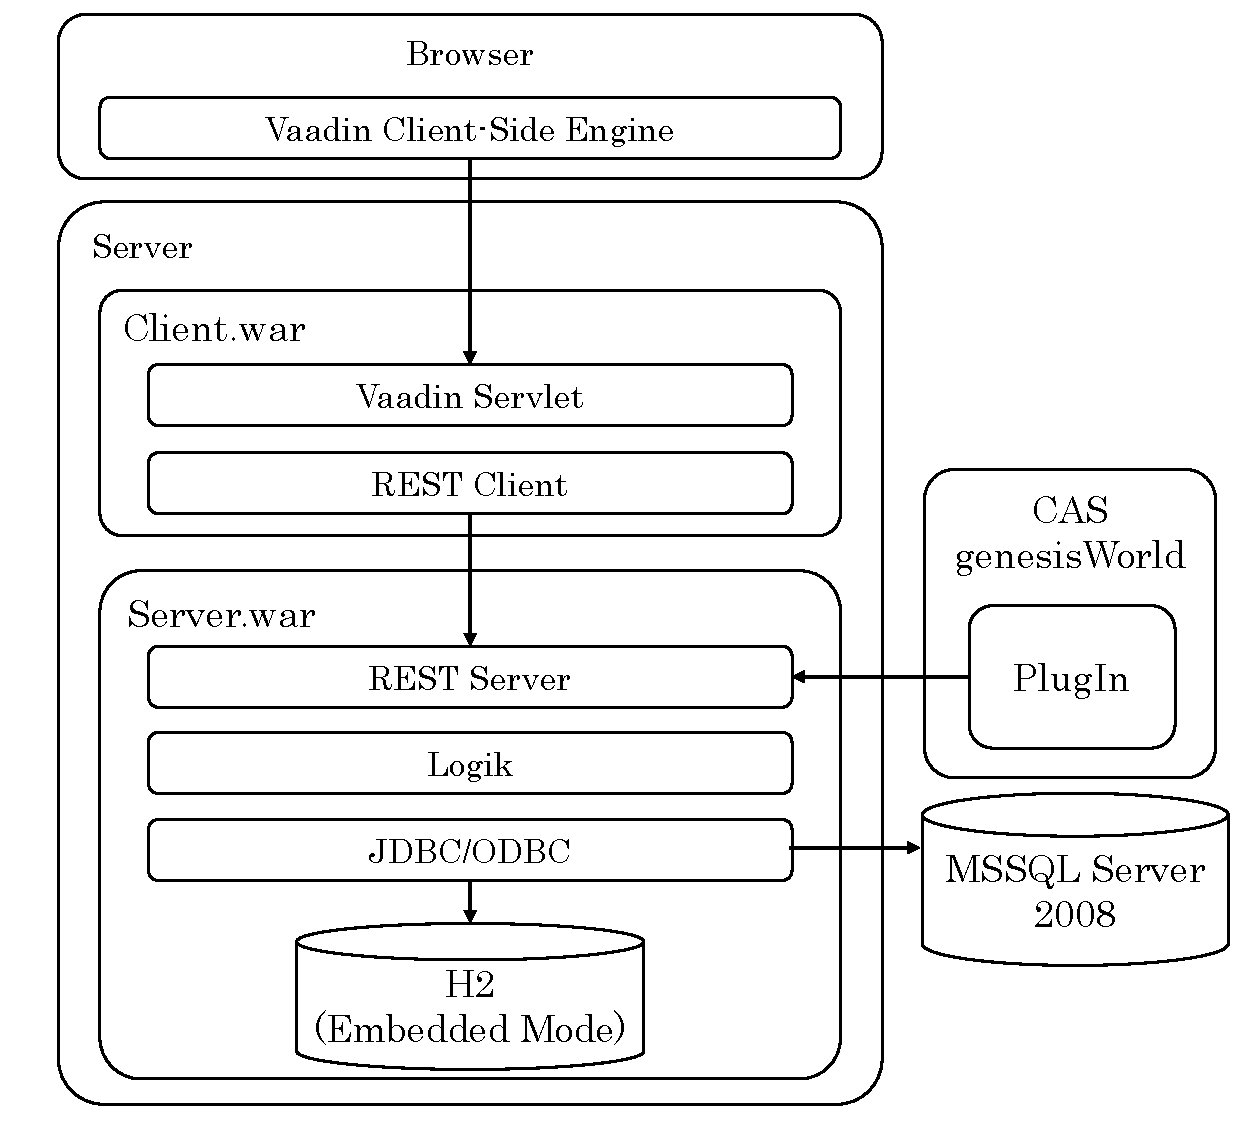
\includegraphics[width=0.8\textwidth, width=0.8\textwidth]{pics/Konzept_architektur.pdf}
\caption{Komponenten des Systems und der Umwelt}
\label{konzept_architektur}
\end{figure} 

\paragraph{Vaadin Client-Side-Engine} Vaadin ist ein auf Java basiertes Webanwendungs-Framework \cite{vaadin2014}. Es bietet eine serverseitige Architektur, wodurch ein Großteil der Programmlogik auf dem Server läuft. Auf der Clientseite baut Vaadin auf dem Ajax-Framework Google Web Toolkit auf und stellt dazu die Client-Side-Engine bereit. Sie verwaltet das Rendering der Oberfläche im Web-Browser.  Dies geschieht durch den Einsatz verschiedener clientseitiger Widgets, die das Gegenstück zu den serverseitigen Vaadin-Komponenten bilden. Es leitet Benutzerinteraktionen an die Serverseite weiter und rendert anschließend die Änderungen für die Benutzeroberfläche. Die Kommunikation findet über asynchrone HTTP-oder HTTPS-Anfragen statt. Weiterhin wird die Komponente durch Vaadin automatisch erzeugt und wird daher für die Umsetzung als gegeben betrachtet.

\paragraph{Client-Webprojekt}

Die Oberfläche des Systems wird durch ein Vaadin-Projekt realisiert. Mit dessen Hilfe werden die Bedien- und Darstellungselemente der Anwendung definiert. Sie ist außerdem für die Interaktion mit dem Benutzer zuständig. Die Delegation von verschiedenen Clients beispielsweise wird von einem Vaadin-Servlet übernommen. Dazu zählt das Empfangen von Anfragen und deren Zuordnung zu einer Sitzung des jeweiligen Benutzers. Die Elemente der Oberfläche selbst werden in Java implementiert. Mithilfe der Java-Klassen wird zur Laufzeit eine Javascript basierte Homepage erzeugt. Die Übersetzung von Java auf Javascript übernimmt Vaadin.

Das Client-Webprojekt wird im ständigen Informationsaustausch mit dem Server-Webprojekt stehen. Die Kommunikation zwischen den beiden Komponenten soll über das REST-Protokoll stattfinden. Dazu implementiert das Client-Webprojekt einen REST-Client. Die Verwendung des REST-Protokolls zwischen dem Client-Webprojekt und Server-Webprojekt stellt überdies ein weiteres Element der losen Kopplung dar.

Ein Prozess in dem die einzelnen Bestandteile Verwendung finden, kann wie folgt aussehen: Die Interaktionen der Benutzer mit der Oberfläche wird Events erzeugen, die zunächst auf der Clientseite durch Widgets verarbeitet werden. Nachfolgend werden die Events durch den HTTP-Server an das Vaadin-Servlet übergeben. Dieser leitet die Events an die entsprechenden Vaadin-Objekte weiter, bis sie zu den in der Anwendung definierten Event-Listenern gelangen. In den Listenern werden anschließend die REST-Clients aufgerufen. Mit Hilfe der REST-Clients werden die Eingaben der Nutzer an das Server-Webprojekt übermittelt. 

\paragraph{Server-Webprojekt}

Die eigentliche Lösung der Problemstellung soll im Server-Webprojekt des Softwaresystems implementiert werden. Es soll vollständig auf Java basieren. In ihr werden sich Klassen und Methoden befinden die eine Ermittlung der Informationen aus der H2-Datenbank ermöglichen. Weiterhin soll ein REST-Server implementiert werden, der die Benutzereingaben entgegennimmt. Der REST-Server ist außerdem für die Kommunikation mit dem Plugin zuständig.

Weiterhin wird das Projekt die ETL-Prozessschritte zum Überführen der Daten aus der MSSQL-Datenbank in die H2-Datenbank implementieren. Die genauen Prozessschritte werden in Abschnitt \ref{ch:konzeption:etl} behandelt. 

%Die Logikkomponente in der Architektur stellt eine Zusammenfassung aller Funktionen des Anwendungskerns dar. Sie kümmert sich um die Generierung der Abfragen, welche an die Datenbank gestellt werden. Dabei erfolgt eine dynamische Generierung der Abfragen, um nicht durch unnötige Bedingungen die Verarbeitungsgeschwindigkeit zu verringern. Abfragen werden mithilfe der Java Database Connectivity (JDBC) an die Datenbank gestellt. Neben den Funktionen zur Abfragegenerierung enthält die Logikkomponente Prozesse zum Extrahieren und Transformieren von Daten aus der MSSQL-Datenbank. Der ETL-Prozess wird nur einmalig ausgeführt, allerdings stellt er einen wichtigen  Schritt für die Umsetzung dar. 


%In der Server.war werden REST-Requests entgegen genommen. Anhand der mitübertragenen Filteroptionen werden die Bedingungen für die Datenbankabfrage zusammengestellt. Anschließend wird eine Verbindung zur H2-Datenbank aufgebaut. Das Ergebnis der Abfrage wird in das JSON-Format überführt und zurück an die Client.war geschickt. Dort angekommen werden die Daten an die Vaadin-Komponenten übergeben, was einen Neuaufbau der entsprechenden Seitenbereiche bewirkt.      

\paragraph{H2-Datenbank}

Die H2-Datenbank wird als ein Bestandteil des Server-Webprojektes eingesetzt. Dies wird durch den Betrieb der H2-Datenbank im Embbeded-Modus erreicht. Dadurch werden Verzögerungen vermieden, die bei der Kommunikationen über ein Netzwerk entstehen können. Um möglichst kurze Antwortzeiten zu erreichen wird die In-Memory-Variante der Tabellen verwendet.

\paragraph{CAS genesisWorld Plugin} Systeme die auf dem Datenbestand anderer Systeme aufbauen können zwei verschiedene  Ansätze zur Sicherstellung ihrer Aktualität verfolgen. Unser nebenläufiges System bezeichnen wir als A und den CAS genesisWorld Anwendungsserver als B. Einer der Ansätze ist die Intervall basierte Nachfrage über Veränderungen von A. Hierbei fragt A bei B zu festgelegten Zeitpunkten nach, ob Daten verändert wurden. Die Definition eines optimalen Intervalls stellt eine der größten Schwierigkeiten dar. Ist der Intervall zu groß, sinkt die Aktualität des Datenbestandes. Ist er zu klein, entsteht eine starke Belastung für B. Der andere Ansatz ist A über Veränderungen an den Datensätzen von B zu informieren. Dadurch werden keine unnötigen Abläufe angestoßen, da nur im Falle einer Manipulation eines Datensatzes Prozesse in Bewegung gesetzt werden. Der zweite Ansatz ist zwar effizienter, allerdings nicht immer umsetzbar. Das kann technische oder unternehmenspolitische Gründe haben, die notwendige Veränderung am Legacy-System  ausschließen.  

In CAS genesisWorld gibt es die Möglichkeit den zweiten Ansatz umzusetzen. Die Idee dabei ist den CAS genesisWorld Anwendungsserver um ein Plugin zu erweitern, welches über Veränderungen in den Datensätzen benachrichtigt wird. Das Plugin soll über einen REST-Client die \textit{GGUID} des betroffenen Datensatzes an das Server-Webprojekt senden. Dort soll eine Kontrolle stattfinden, die den Datensatz auf Relevanz überprüft. Wird eine Relevanz festgestellt besorgt sich das Server-Webprojekt, anhand der zuvor übermittelten GGUID, alle benötigten Daten.

%% ===========================
\section{Datenbankdesign}
%% ===========================

Das Datenbankdesign stellt einen wichtigen Abschnitt in der Konzeption dar. An dieser Stelle werden Festlegungen im Bereich des Datenmodells getroffen. Sie entscheiden, ob Anforderungen und Erwartungen erfüllt werden können. Weiterhin werden die Charakteristika der aufzubewahrenden Daten untersucht und das Datenmodell entsprechend nach ihnen gestaltet.

%% ===========================
\subsection{Konzeptionelles Modell}
%% ===========================

Zunächst wird mithilfe eines konzeptionellen Modells eine Übersicht der zu verwaltenden Daten aufgezeigt. Das Modell bietet durch einen hohen Abstraktionsgrad einen idealen Einstieg in das geplante Vorhaben. In Abbildung \ref{konzept_erd} ist das Modell in Form eines ERD-Diagramms dargestellt. 

Im Mittelpunkt stehen in diesem Fall die Personen. Diese besitzen jeweils eine eigene Adresse mit ihren Kontaktdaten. Personen können außerdem zu Gruppen gehören, müssen aber nicht zwangsweise einer zugeordnet werden. Neben der Adresse erzeugen Personen ihre eigenen CRM-Objekte. Diese können sie mit anderen Personen teilen, wodurch ein CRM-Objekt zu mehreren Personen in Beziehung treten würde. CRM-Objekte wiederum können in verschiedenen Ausprägungen z.B. als E-Mail oder Dokument auftreten. Die Ausprägungen besitzen verschiedene Attribute welche es ermöglichen das CRM-Objekt einem Zeitpunkt zuzuordnen.

\begin{figure}[htbp]
\centering
  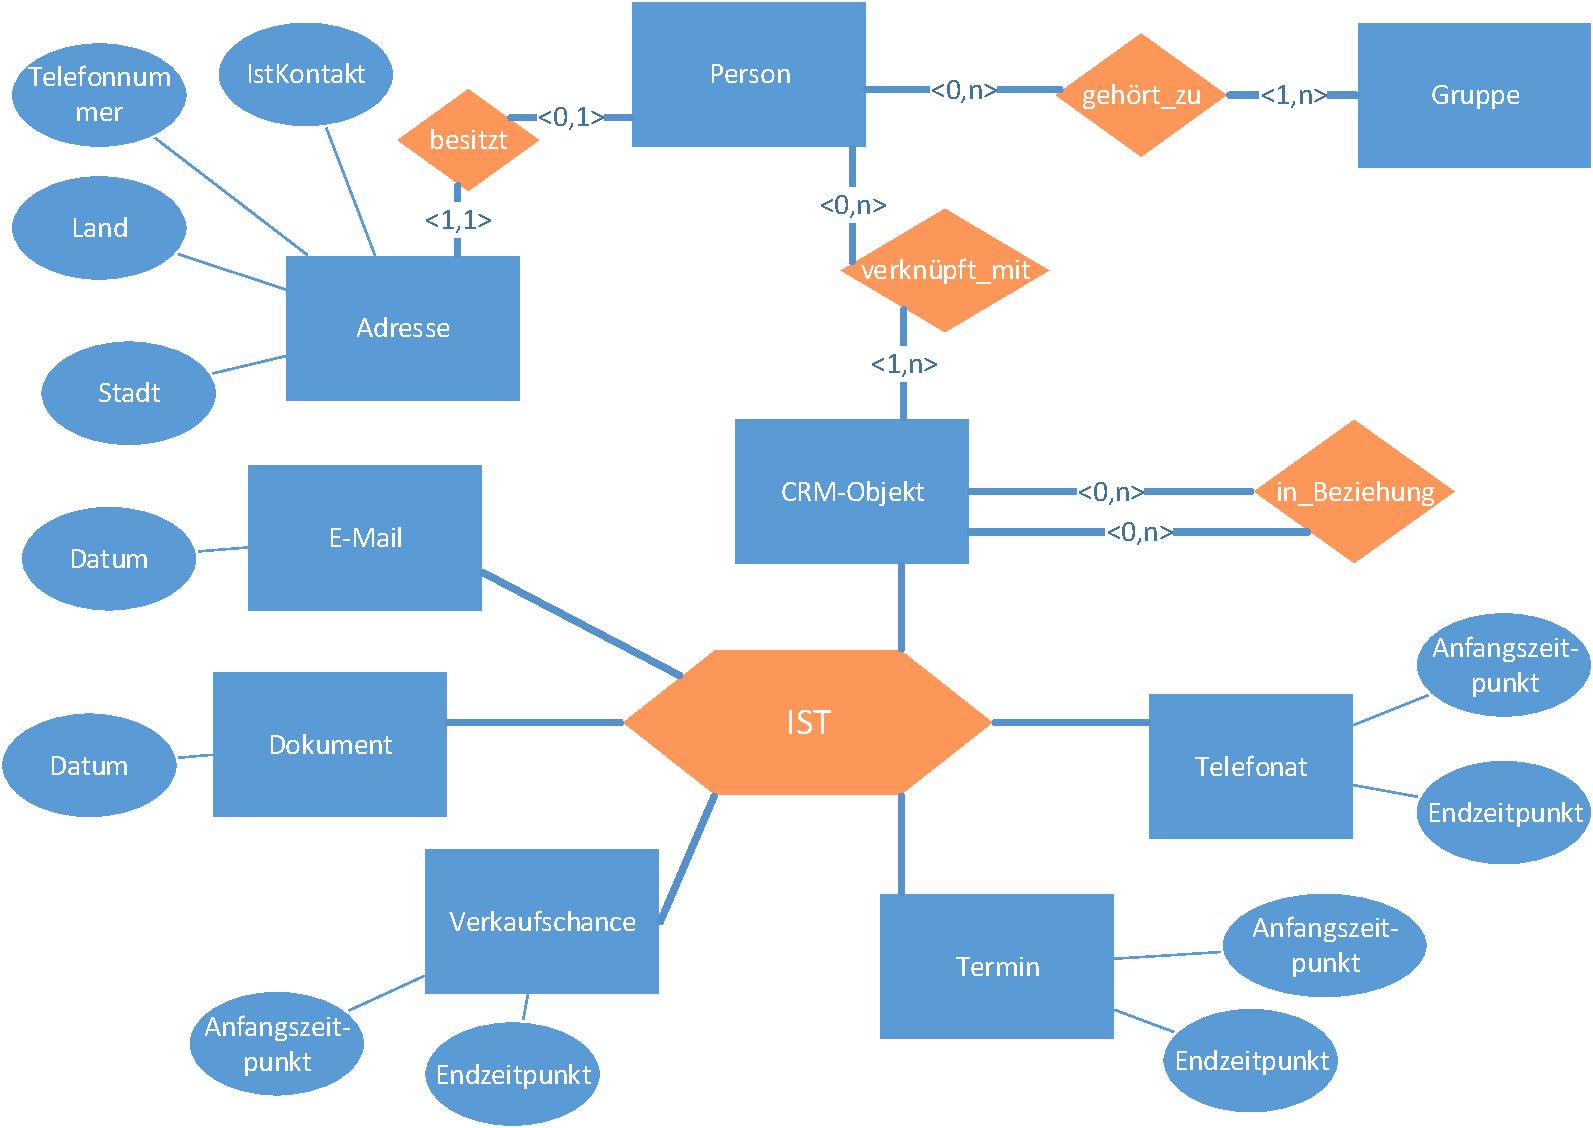
\includegraphics[width=1.0\textwidth, width=1.0\textwidth]{pics/konzept_erd.pdf}
\caption{ER-Modell als Darstellungsform des Konzeptionelles Modell}
\label{konzept_erd}
\end{figure} 

%% ===========================
\subsection{Datenbankschema}
%% ===========================

Zunächst wird auf das geplante Schema eingegangen welches in der H2-Datenbank eingesetzt wird. Indessen werden die Überlegungen und Entscheidungen die zur Entstehung des Schemas geführt haben erläutert. 

Zuerst werden Überlegungen hinsichtlich der Normalisierung angestellt. Die Normalisierung bietet dem Designer die Möglichkeit einen Austausch zwischen Performance und Stabilität vorzunehmen \cite{geisler2011datenbanken}. Im neuen System stellt ersteres absolute Priorität dar. Aus diesem Grund hat eine Normalisierung keine besonders hohe Priorität.

Abbildung \ref{konzept_SchemaNeu} zeigt das für die Datenbank neu entworfene Schema. 

\begin{figure}[htbp]
\centering
  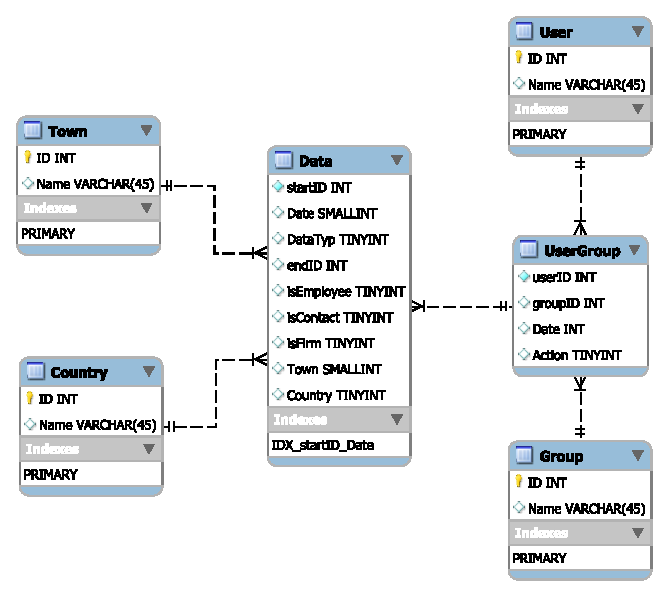
\includegraphics[width=0.8\textwidth, width=0.8\textwidth]{pics/NewSchema.pdf}
\caption{Neues Datenbankschema}
\label{konzept_SchemaNeu}
\end{figure} 

Die zugrundeliegende Idee ist alle Informationen über die Beziehung zwischen den Personen und den CRM-Objekten in der \textit{Data}-Tabelle aufzubewahren. Dadurch liegt ein wesentlich geringer normalisiertes Schema vor als in der MSSQL-Datenbank. Jede Tupel repräsentiert dabei ein CRM-Objekt, das zwei Personen in Beziehung zueinander setzt. Außerdem soll jede Tupel einem Tag zugeordnet werden.

Die erste und vierte Spalte \textit{startID} beinhalten jeweils die ID der Personen. Eine Zuordnung der Tupel zu einem Datum erfolgt über die Spalte \textit{Date}. Um CRM-Objekte zu unterscheiden, werden Zahlen von eins bis fünf in der Spalte \textit{DataTyp} für die jeweiligen Ausprägungen des CRM-Objektes vergeben. Alle anderen Spalten, wie \textit{Town} oder \textit{Country} beinhalten Werte, anhand denen die Ergebnismenge verringert werden kann. 

Um mit den geringeren Kapazitäten des Hauptspeichers zurechtzukommen, wird auf das Problem der Datenredundanz eingegangen. Durch Normalisierung lässt sich Datenredundanz zwar verringern, allerdings steigt dadurch der Aufwand zur Wiedergewinnung der Daten. Im neuen Schema werden solche Maßnahmen auf die Spalte \textit{Town} und \textit{Country} angewendet. 

Die Tabelle \textit{Data} wird voraussichtlich Millionen von Tupeln besitzen, weshalb Möglichkeiten in der Normalisierung in Betracht gezogen werden. Beispielsweise werden sich die Ländernamen sehr oft wiederholen. Der Datentyp Varchar benötigt pro Zeichen 2 Byte an Speicherplatz. Aufgrund der stetigen Wiederholung von gleichen Wörtern ist die Verwendung von Varchar an dieser Stelle ungeeignet. Angesichts dessen sollen die Ländernamen in einer eigenen Tabelle aufbewahrt werden. 

Die Normalisierung würde zum Beispiel bei dem Wort "Deutschland" eine Reduktion von 22 Byte auf 1 Byte bewirken. Die Reduzierung auf 1 Byte entsteht durch die Verwendung des Datentyps tinyint. Diese Schritte zur Normalisierung werden ebenfalls für die Spalte \textit{Town} angewandt. Bei ihr wird allerdings der Datentyp smallint verwendet, da dessen Zahlenbereich von $-32768$ bis $32767$ reicht. Damit lassen sich alle Städte aus der MSSQL-Datenbank abdecken. 

Die Spalten \textit{isEmployee}, \textit{isContact} und \textit{isFirm} können nur zwei verschiedene Zustände darstellen. Trifft zu oder trifft nicht zu. Der Datentyp bool ist daher ausreichend zur Abbildung der  Zustände. Ein Feld vom Datentyp datetime benötigt 8 byte an Speicher. Um hier ebenfalls Einsparungen vorzunehmen, wurde beschlossen das Datum als smallint zu deklarieren. Dies ist möglich, weil nur der Tag des Datums von Interesse ist. Dazu wird ein frei gewählter Zeitpunkt Null festgelegt. In unserem Fall wurde der 01.01.1990 als Zeitpunkt gewählt, da keine älteren Daten existieren, die eine Relevanz besitzen. Der Wert eines Datums wird durch die Anzahl der Tage seit dem Zeitpunkt Null ermittelt. Ein Beispiel wäre der 05.01.1990 der in der Spalte \textit{Date} als eine 4 vermerkt werden würde. Die Hochrechnung der Tabelle \ref{tb_speicherplatzverbrauch} zeigt, dass durch die Normalisierung der Speicherplatzverbrauch auf $ \frac{1}{6} $ gesenkt werden kann.

\begin{table}[htbp]
\centering
\begin{tabulary} {\linewidth} {l  r  C  l  C  r}
& & & & & \\
\multicolumn{6}{l}{Speicherplatzverbrauch ohne Normalisierung}\\
& & & & & \\
Zeitpunkt(timestamp) & 8 byte & x & 18.000.000 & = & \textasciitilde 137 MB \\  
Stadt(varchar) & 16 byte & x & 18.000.000 & = & \textasciitilde 343 MB \\  
Land(varchar) & 20 byte & x & 18.000.000 & = & \textasciitilde 274 MB \\  
\midrule
& & & & Summe & \textasciitilde 754 MB\\
& & & & & \\
\multicolumn{6}{l}{Speicherplatzverbrauch mit Normalisierung}\\
& & & & & \\
Zeitpunkt(smallint) & 2 byte & x & 18.000.000 & = & \textasciitilde 34 MB \\  
Stadt(integer) & 4 byte & x & 18.000.000 & = & \textasciitilde 72 MB \\  
Stadt(varchar + tinyint) & 16 byte & x & 21.000 & = & \textasciitilde 0,32 MB \\  
Land(tinyint) & 1 byte & x & 18.000.000 & = & \textasciitilde 17 MB \\  
Land(varchar + tinyint) & 20 byte & x & 218 & = & \textasciitilde 0,004 MB \\
\midrule  
& & & & Summe & \textasciitilde 123 MB\\
& & & & & \\
\end{tabulary}
\caption{Vergleich des Speicherplatzverbrauchs}
\label{tb_speicherplatzverbrauch}
\end{table}

Durch die Normalisierung kann zwar Speicherplatz gespart werden doch nun muss überlegt werden wie die Informationen wiederbeschafft werden sollten. Wird eine Benutzerabfrage gestellt die eine Filterung anhand einer Stadt voraussieht, wird zuerst die \textit{ID} der Stadt benötigt. Dabei können zwei verschiedene Ansätze verfolgt werden. Der erste Ansatz wäre ein Verbund zwischen \textit{Town} und \textit{Data}, um direkt mit dem Namen der Stadt zu arbeiten. Eine andere Möglichkeit wäre eine separate Abfrage an die Datenbank zu stellen, in der die \textit{ID} zum Namen ermittelt wird. Mithilfe der \textit{ID} kann dann ohne einen Verbund die Ergebnismenge ermittelt werden. Dieser Ansatz dürfte zu geringeren Antwortzeiten führen, da keine Netzwerkverzögerungen existieren. Überdies findet der Zugriff mittels geeigneter Indizierung und auf In-Memory-Tabellen statt, was die Antwortzeit ebenfalls verkürzt. Diese Vorgehen können für die Stadt, das Land und die Gruppenzugehörigkeit angewendet werden.

Die Tabelle \textit{GroupDate} unterscheidet sich von den anderen Tabellen wie \textit{Town} oder \textit{Country}, da in dieser noch weitere Details vermerkt sind. Diese ermöglichen es die Personenkonstellation innerhalb der Gruppen über die Zeit hinweg nachzuvollziehen. In der Spalte \textit{Action} wird festgelegt, ob die Tupel einen Eintritt oder einen Austritt einer Person darstellt. Die Spalte \textit{Date} beinhaltet das Datum des Ereignisses. Mithilfe beider Attribute lassen sich Gruppenzusammensetzung auf bestimmte Zeitpunkte bezogen rekonstruieren.

%% ===========================
\subsection{Zugriffsstrukturen}
%% ===========================

Zum Beschleunigen der Zugriffe auf die Datensätze der H2-Datenbank wird auf die beabsichtigten Zugriffsverfahren eingegangen. 

Indizes werden zur Beschleunigung von Suchen nach bestimmten Spaltenwerten eingesetzt. Ohne Indizes müsste die H2-Datenbank beim ersten Datensatz beginnen und dann die gesamte Tabelle durchgehen, um eine Abfrage zu beantworten. Je größer die Tabelle ist, desto höher ist der Aufwand dafür. Der Einsatz von Indizes ist in Anbetracht der Zielsetzung von kurzen Antwortzeiten ein unerlässliches Hilfsmittel. Jeder Index bedeutet allerdings einen Zuwachs im Speicherplatzverbrauch, was bei In-Memory-Datenbanken zu berücksichtigen ist. Deshalb werden nur absolut notwendige Indizes erzeugt. Außerdem führen Indizes zu einem erhöhten Aufwand bei Aktualisierungen, da neben den Datensätzen auch ihre Indizes aktualisiert werden müssen. Zur Indexierung der Tabellen \textit{Town}, \textit{UserGroup}, \textit{Country}, \textit{User} und \textit{Group} eignen sich Hash-Indizes. Sie bieten einen extrem schnellen Zugriff auf die Daten. Diese Schnelligkeit ergibt sich aus der Verwendung von Berechnungsvorschriften zur Ermittlung der Position des gesuchten Wertes  \cite{SWB-352401869}. Indizierungen sollen im vorliegenden Schema über die Spalten mit der Bezeichnung \textit{Name} vorgenommen werden, da der Client mit dem Namen anstatt mit der ID arbeitet. Mithilfe des Namens wird anschließend die zugehörige ID ermittelt. Die Nutzung von Hash-Indizes bringt allerdings Limitierungen mit sich. Eine der wichtigsten ist, dass sie nur für Vergleiche ("=") verwendbar sind. Somit werden keine Wertebereichabfragen ("<" oder ">") unterstützt.

Für die Tabelle \textit{Data} eignet sich der B\textsuperscript{+}-Baum-Index. Er ermöglicht eine effizientere Ausführung der Grundoperationen wie Suchen, Einfügen und Löschen. Die Spalte \textit{startID} und \textit{Date} eignen sich am besten für die Indexierung. Das erste Attribut auf das bei der Suche zugegriffen wird ist die \textit{startID}, da sie die Personen beinhaltet von der aus die Beziehungen ermittelt und bewertet werden. Der zweite Zugriffswert (\textit{Date}) eignet sich aufgrund der Tatsache, dass immer bestimmte Zeitspannen betrachtet werden. Sind die Werte der Spalte sortiert, können durch Bereichsabfragen sehr schnell alle Tupeln zwischen dem Start- und Endzeitpunkt ermittelt werden. Dabei handelt es sich um einen Mehr-Attribut-Index, da wir zwei Attribute verwenden. Der Vorteil eines Mehr-Attribut-Index ist, dass bei einer Punkt-Abfrage über alle Zugriffsattributwerte nur ein Indexzugriff erfolgen muss.

Beide Spalten sind sortiert und bieten sich somit für die Verwendung von einem geclusterten Index an. Ein geclusterter Index ist in der gleichen Form sortiert wie die interne Relation. Dadurch bietet er eine sehr gute Unterstützung für Bereichsabfragen.


%% ===========================
\section{ETL-Prozess}
\label{ch:konzeption:etl}
%% ===========================

Daten der operativen Systeme unterstützen die wertschöpfenden Geschäftsprozesse innerhalb eines Unternehmens. Sie sind demnach auf die Steuerung und Überwachung des Tagesgeschäftes ausgerichtet und daher transaktionsbezogen. Die Daten sind aufgrund ihres eigentlichen Verwendungszwecks in ihren Begrifflichkeiten häufig nicht vergleichbar und ihrer Bewertung sowie Konsolidierung unterschiedlich. Um die Daten dennoch für unsere Bewertung einzusetzen, ist eine Überführung in eine geeignete Struktur von Vorteil. Eine solche Überführung wird in der Literatur als Extract-Transform-Load (ETL)-Prozess bezeichnet \cite{ElSappagh201191}. 

Abbildung \ref{konzept:etl} zeigt das erarbeitete Konzept zur Umsetzung eines solchen ETL-Prozesses. In den nächsten drei Abschnitten werden die ETL-Schritte näher erläutert.

\begin{figure}[htbp]
\centering
  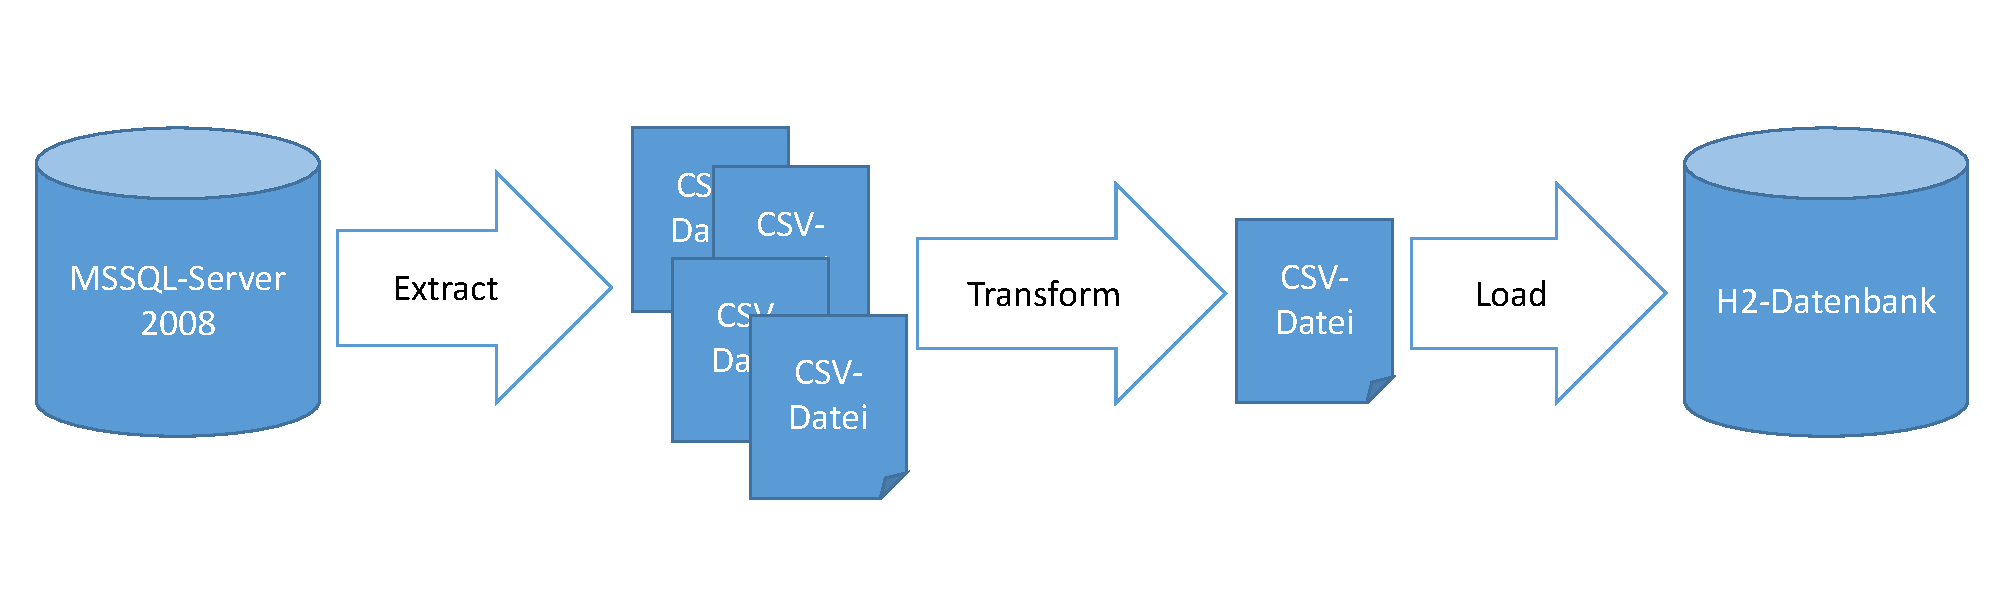
\includegraphics[width=1.0\textwidth, width=1.0\textwidth]{pics/ETL.pdf}
\caption{ETL-Prozess}
\label{konzept:etl}
\end{figure} 


%% ===========================
\subsection{Extract}
\label{ch:konzeption:etl:extract}
%% ===========================

Zunächst dient die Extraktion primär der Beschaffung von Daten aus der MSSQL-Datenbank. Überdies können durch den Prozess Daten bereits reduziert,  zusammengeführt und ersetzt werden. Für eine zutreffende Formulierung der Abfragen müssen Besonderheiten im Ermitteln der Daten beachtet werden. Eine solche Besonderheit wäre beispielsweise zwei Spalten mit unterschiedlichen Formaten bei dem Datum.

In der Extraktion sollen SQL-Abfragen formuliert werden mit denen die Daten aus der MSSQL-Datenbank in die H2-Datenbank überführt werden können. Dabei gilt es die Abfragen so zu formulieren, dass die Struktur des Abfrageergebnisses der Tabelle des neuen Schemas entspricht.

Weiterhin sind Besonderheiten in der Extraktion zu beachten. Es existieren Datensätze in der MSSQL-Datenbank die sich über längere Zeiträume erstrecken. Beispielsweise erstrecken sich Termine wie Tagungen über mehrere Tage. In der MSSQL-Datenbank werden diese Termine in einer Tupel aufbewahrt. Bei unserer Analyse hingegen stellt jede Tupel eine Verknüpfung zwischen Personen zu einem bestimmten Tag dar. Somit muss ein Datensatz der sich über mehrere Tage erstreckt, in der H2-Datenbank durch mehrere Tupeln repräsentiert werden. Aufgrund dessen wird im Ergebnis der SQL-Abfrage die Zeitspanne eines CRM-Objektes in Tagen vermerkt. In späteren Transformationen kann mithilfe dieser Angabe die entsprechende Anzahl an Tupeln erzeugt werden.

Eine weitere Besonderheit ergibt sich durch eine Funktionalität von CAS genesisWorld, welche es ermöglicht Termine auf andere Zeitpunkte zu verschieben. Diese Funktion wird von manchen Nutzern missbraucht. Anstatt für einen ähnlichen Termin einen neuen Eintrag anzulegen, wird ein alter Termin aus Bequemlichkeit geschoben. Das hat zur Folge, dass Termine die tatsächlich stattgefunden haben, in der Datenbank nicht mehr existieren. Um trotzdem diese Termine zu berücksichtigen wurde folgendes Konzept erarbeitet. 

Dem \textit{Changelogbook} lassen sich Veränderungen von Feldern entnehmen. Um Schiebungen zu erkennen werden die Änderungen in den Spalten \textit{start\_dt} und \textit{end\_dt} benötigt. Zur Feststellung ob ein Termin stattgefunden hat und anschließend geschoben wurde, müssen drei Bedienungen erfüllt sein. Die erste ist der Zeitpunkt der Schiebung, der nach dem Termin liegen muss. Wird ein Termin aus anderen Gründen geschoben findet dies in der Regel vor dem Start des Termins statt, damit die Personen nicht unnötig zum Termin erscheinen. Die zweite Bedingung ist, dass der neue Termin in der Zukunft liegen muss. Neben den beiden zuvor genannten Bedingungen muss die Operation auf den Datensätzen ein Update gewesen sein. Nur dann ist der Datensatz von Relevanz für die Ermittlung der geschobenen Termine. 

Die Ergebnisse sämtlicher Extraktionen werden in CSV-Dateien abgespeichert. Damit werden unteranderem nachvollziehbare Zwischenergebnisse erzeugt, die z.B. bei Fehlersuchen hilfreich sind. Weiterhin wird die Belastung für das  Systems verringert, da nicht alle Ergebnisse bis zum Ende der Extraktion in der Java-Laufzeitumgebung aufbewahrt werden müssen.

%% ===========================
\subsection{Transform}
%% ===========================

Zu Beginn der Transformation werden Filterungen durchgeführt. Unter der Filterung von operativen Daten versteht man eine Bereinigung syntaktischer oder inhaltlicher Defekte, der zu übernehmenden Daten. Die MSSQL-Datenbank besteht zu 37\% aus Nullwerten und zu 4\% aus Feldern mit ausschließlich Leerzeichen. Daten die beispielsweise Nullwerte enthalten und für die Ermittlung des Datums benötigt werden, sind für die Analyse nicht zu gebrauchen. Sie können daher im Laufe des Prozesses aus den Daten entfernt werden. Bei den anderen Filteroperationen können Nullwerte vernachlässigt werden, da sie zweckmäßig abdingbar sind.

Der nächste Schritt ist die Harmonisierung der Daten. Unter anderem besitzen die Telefonnummern kein einheitliches Format. Sie wurde manuell von Sachbearbeitern eingetragen. Zur Lösung des Problems werden aller Nummern in ein einheitliches Format gebracht, welches einen automatischen Vergleich ermöglicht. Dies geschieht durch vordefinierte Regeln. Die verschiedenen Variationen werden durch händische Untersuchungen ermittelt. Basierend auf den Variationen werden die Regeln zur Transformation festgelegt. Die verschiedenen Ausprägungen von CRM-Objekten müssen ebenfalls in eine einheitliche Struktur gebracht werden. Sie besitzen alle die benötigten Informationen, allerdings werden diese unter unterschiedlichen Bezeichnungen und eventuell in einem anderen Datenformat aufbewahrt.

Die in der Extraktion genannten Besonderheiten werden durch unterschiedliche Datenbankabfragen ermittelt. Dies führt zu vielen separaten Dateien. Zur Nutzung der Daten werden diese zum Abschluss der Transformation sortiert und zusammengeführt. Das Ergebnis wird anschließend in einer CSV-Datei gespeichert, welche die Basis zum Einspielen der Daten in die H2-Datenbank bildet. Der Grund für das Zusammenzuführen und Sortieren der Dateien liegt in der Wiederverwendung der Datei in anderen Projekten, worauf in der Arbeit allerdings nicht näher eingegangen wird. Außerdem vereinfacht es die Implementierung des Ladeprozesses, da dadurch nur eine Funktion beim Erstellen der Tabelle zu realisieren ist.

%% ===========================
\subsection{Load}
%% ===========================

Beim Laden der Datensätze in die H2-Datenbank soll ein sogenannter "bulk load" verwendet werden. Dieser wird häufig zum Laden von großen Datenmengen aus einer Datei in eine Datenbank eingesetzt. Er ermöglicht ein wesentlich schnelleres Einspielen von großen Datenmengen in die Datenbank, gegenüber der Verwendung von INSERT-Operatoren.

%% ===========================
\section{Entwurf der Oberfläche}
\label{ch:Konzeption:sec:Darstellungskonzepte}
%% ===========================

Beim Entwurf einer Oberfläche ist der Detaillierungsgrad von Informationen ein wichtiger Leitfaden für die Gestaltung. In unserem Fall ist nicht die Eigenschaft eines CRM-Objekts von Interesse, sondern der Typ und dessen Häufigkeit von Beziehungen zu bestimmten Personen. Da keine vertraulichen und sensiblen Daten über die Personen oder die CRM-Objekte aufbewahrt werden, kann jeder Benutzer frei wählen von welcher Person die Bewertung ausgehen  soll. Für die Oberfläche bedeutet dies einen Einstiegspunkt in Form eines Fensters in dem der Benutzername einer Person, von dem die Suche ausgehen soll, eingegeben wird. Zusätzlich werden Felder zum Eintragen der IP-Adresse und Portnummer des Server-Webprojektes angezeigt.

Nach der Anmeldung wird eine neue Seite aufgebaut, in der das Ergebnis der Analyse zu sehen ist. Dessen Aufbau ist in Abbildung \ref{konzept_darstellung} zu sehen. Im oberen Bereich auf der Seite sind alle Regler, CheckBoxen und Eingabefelder zur Filterung der Ergebnismenge zu finden. Direkt darunter befindet sich ein Diagramm, welches das Ergebnis der Abfrage visualisieren soll.

\begin{figure}[htbp]
\centering
  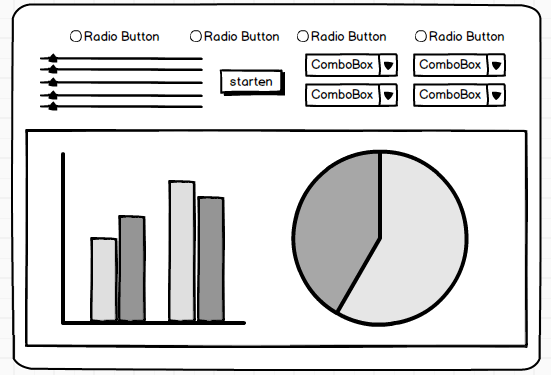
\includegraphics[width=0.8\textwidth, width=0.8\textwidth]{pics/mockup.png}
\caption{Entwurf der Oberfläche}
\label{konzept_darstellung}
\end{figure} 

Bei der Wahl eines Diagrammtyps ergeben sich durch das verwendete Framework allerdings Einschränkungen. Im Grunde lässt sich jede Darstellung umsetzen, jedoch ist das Aufwand-Nutzen-Verhältnis zu berücksichtigen. Beispielsweise wäre in diesem Fall die Entwicklung eines eigenen Diagramms mit einem Aufwand verbunden der den geringen Mehrwert nicht rechtfertigen würde. Daher werden nur mit dem Framework umsetzbare Diagrammtypen betrachtet. In einer Vorauswahl wurden einige  Typen ausgewählt, die in Abbildung \ref{konzept_darstellung2} dargestellt sind. 

Netzdiagramme (a) geben Eigenschaften verschiedener Systeme wieder. Sie eignen sich daher gut zur Darstellung von Ausprägungen. Für die vorliegenden Daten ist diese Darstellung gänzlich ungeeignet, da Mengen betrachtet werden. 

Mithilfe von Liniendiagrammen (b) lassen sich Trends und Zeitreihen darstellen. Die Verwendung verschiedener Linien ermöglicht zudem die Darstellung mehrerer Trends. Die Benutzung dieses Diagramms wäre nicht sinnvoll, da die Ergebnismenge sich nicht auf verschiedene Zeitpunkte bezieht, sondern die Summe der Werte aus einer Zeitreihe beinhaltet.

\begin{figure}[htbp]
\subfigure[Netzdiagramm]{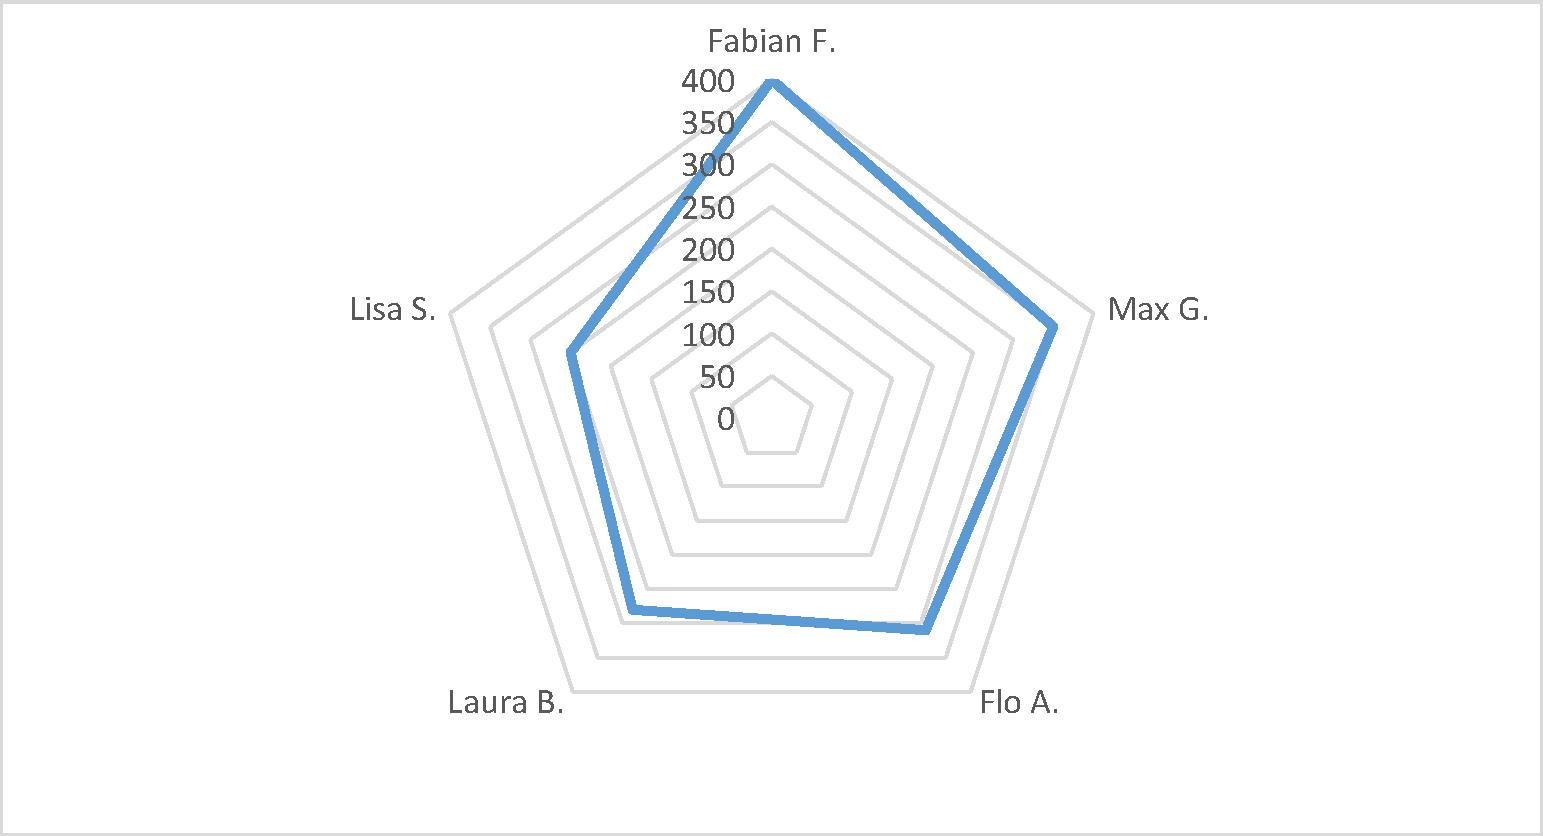
\includegraphics[width=0.3\textwidth]{pics/konzept_netzdiagramm.pdf}}\hfill
\subfigure[Liniendiagramm]{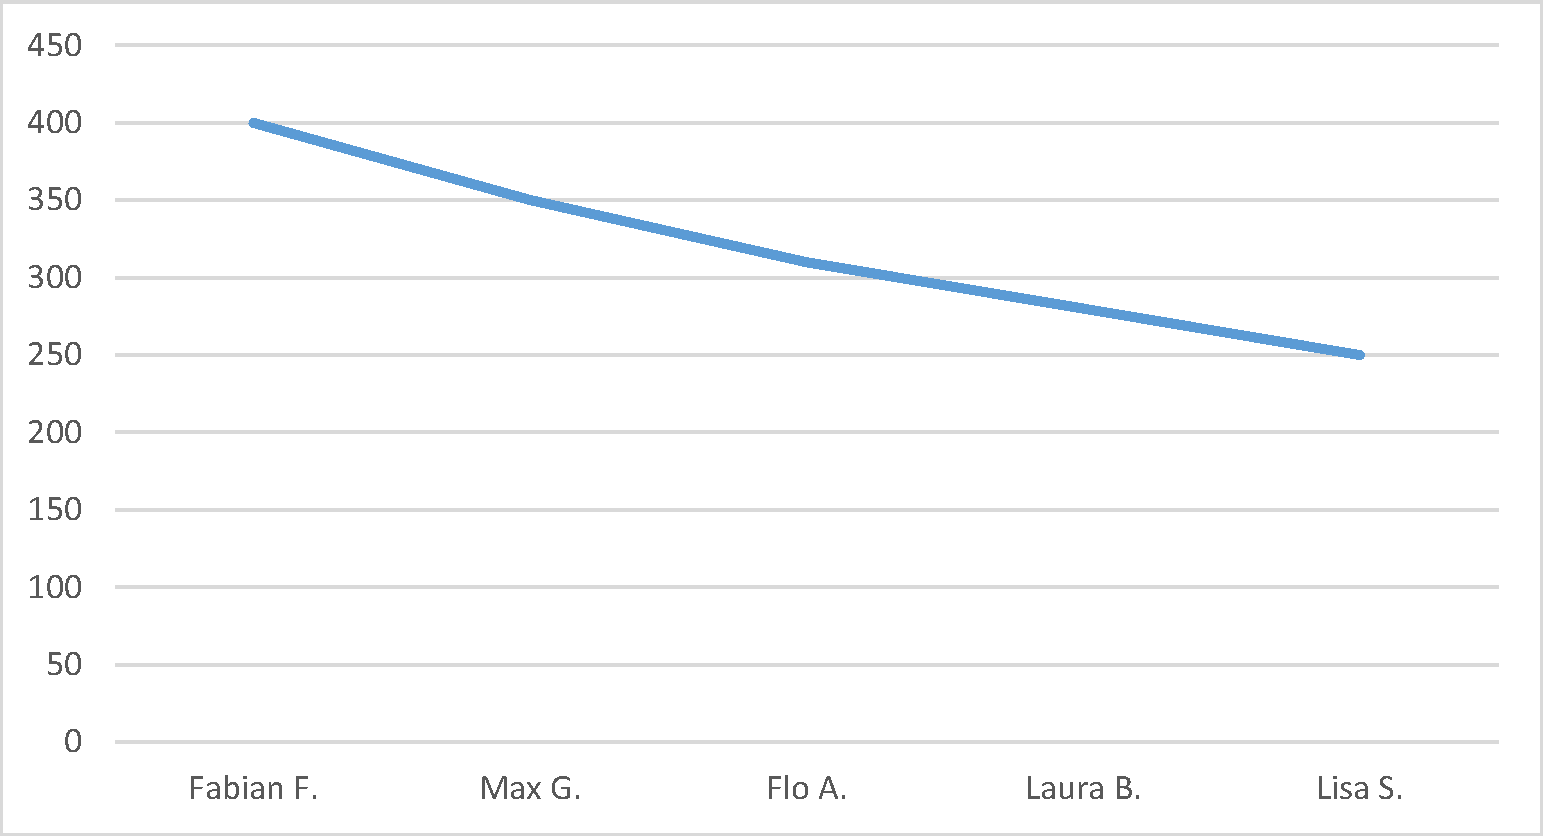
\includegraphics[width=0.3\textwidth]{pics/konzept_liniendiagramm.pdf}}\hfill
\subfigure[Tree Map]{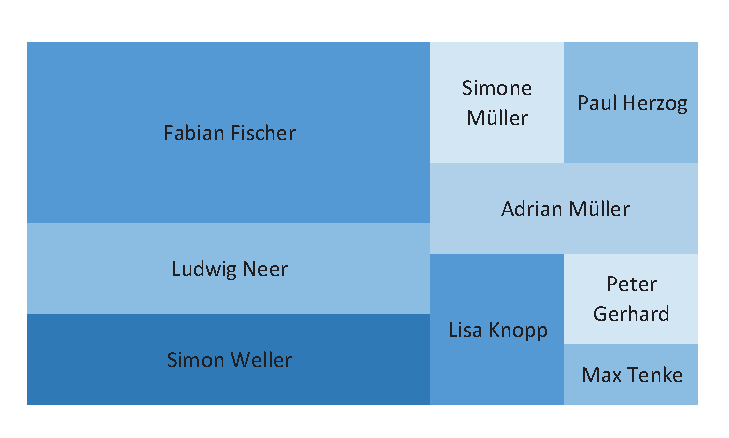
\includegraphics[width=0.3\textwidth]{pics/konzept_tree_map.pdf}}\hfill
\subfigure[Tortendiagramm]{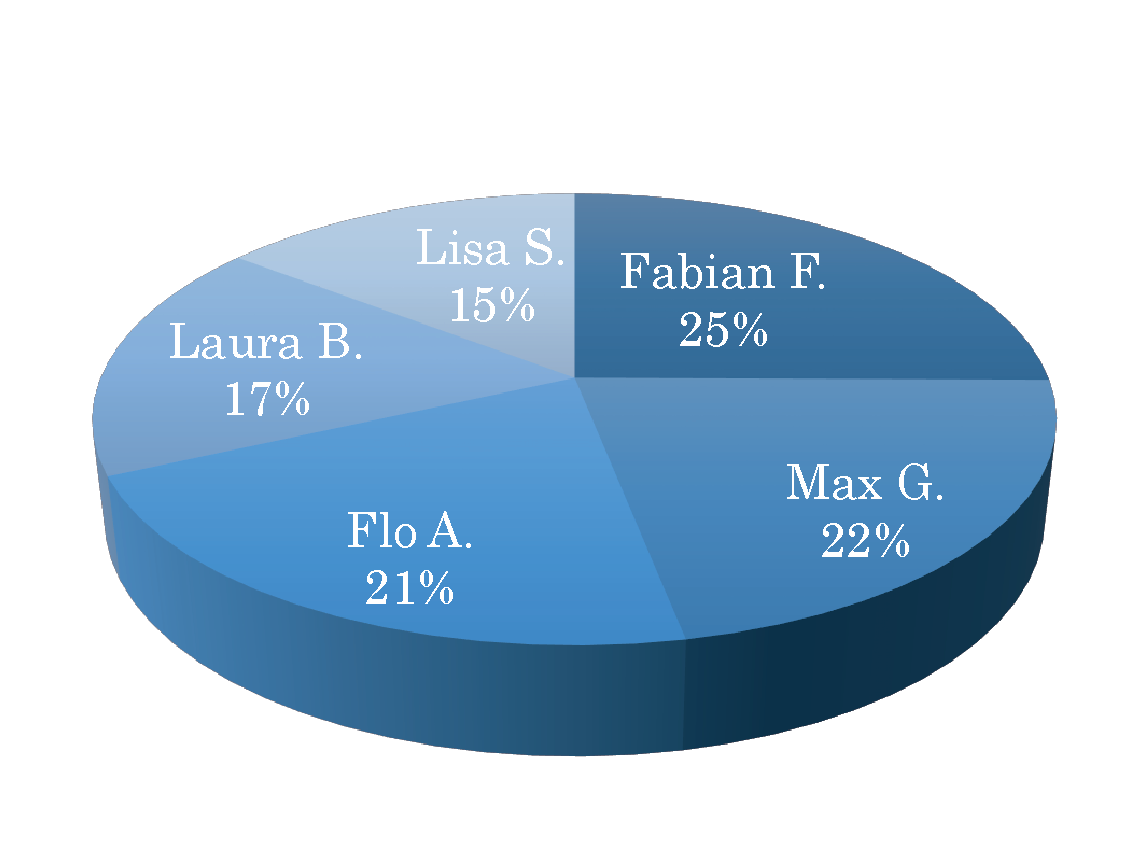
\includegraphics[width=0.3\textwidth]{pics/konzept_tortendiagramm.pdf}}
\subfigure[Balkendiagramm]{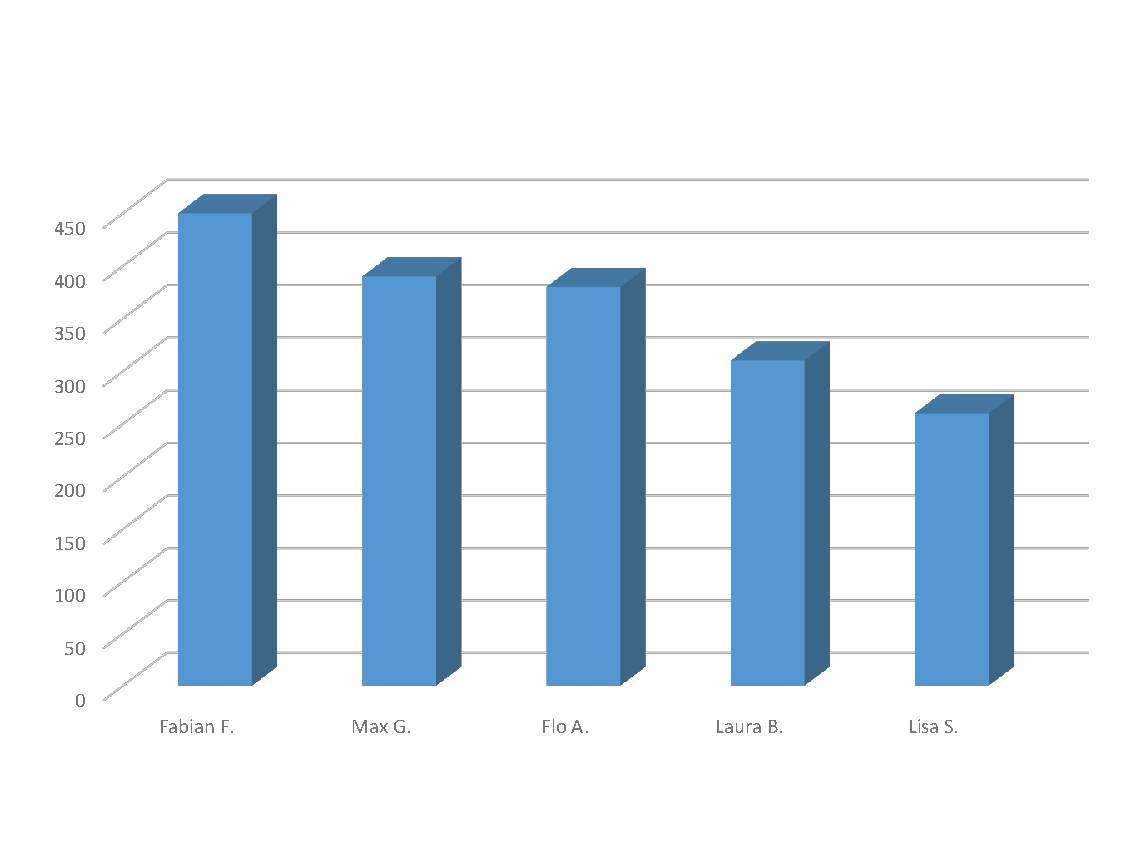
\includegraphics[width=0.3\textwidth]{pics/konzept_balkendiagramm.pdf}}
\caption{Entwürfe für die Oberfläche}
\label{konzept_darstellung2}
\end{figure}

Bei einer Tree Map (c) steht jede Fläche eines Rechtecks im proportionalen Zusammenhang zur Gesamtfläche. Die Beachtung von Größenverhältnissen stellt eine nützliche Eigenschaft für unsere Daten dar. In unserem Fall würde jedes Rechteck die Summe der CRM-Objekte einer Person darstellen. Diese könnten wiederum in weitere Rechtecke unterteilt werden oder mithilfe eines Drilldowns
\footnote{Als Drilldown wird im Allgemeinen die Navigation in hierarchischen Daten bezeichnet. Auf Oberflächen bezogen wird damit die Darstellung von Detailinformationen durch einem Klick auf Darstellungselemente ausgedrückt.}
 die Anteile der unterschiedlichen CRM-Objekte aufzeigen. Eine weitere Unterteilung der Rechtecke würde allerdings aufgrund zu vieler Kacheln schnell zu einer schlechten Übersicht führen. Wird in einer Tree Map die Drilldown-Navigation gewählt, ist die Übersicht aller Informationen auf einen Blick nicht mehr gegeben. Aufgrund der Nachteile in der jeweiligen Variation wurde sich gegen den Einsatz einer Tree Map entschieden.

Kreisdiagramme (d) ermöglichen eine Betrachtung der Gesamtheit zu ihren Einzelstücken, da der Kreis ein geschlossenes System darstellt. Allerdings müssen sich alle Kreisstücke auf die gleiche Basis beziehen. Es eignet sich hervorragend zur Darstellung von Verhältnissen. Wird nun eine weitere Unterteilung der Teilwerte benötigt, geht die Übersicht verloren. Um das zu vermeiden wird die unterteilte Teilmenge häufig in separaten Ansichten dargestellt. Allerdings steigt dadurch der Aufwand für den Nutzer in der Bedienung des Systems. 

Das Balkendiagramm (e) ist für die Darstellung der Daten am geeignetsten. Reihenfolgen lassen sich beispielsweise durch die resultierenden Stufen sehr gut darstellen. Balken selbst lassen sich außerdem in einzelne Teile aufspalten, ohne die Übersichtlichkeit zu verringern. Gegenüber dem Kreisdiagramm bietet es zwar eine schlechtere Betrachtung des Gesamten zu den Einzelstücken, allerdings ist das in diesem Anwendungsfall auch nicht problematisch. Es ist vielmehr von Bedeutung die Ergebnisse in Form eines Rankings darzustellen.

%% ===========================
\section{Technologien}
%% ===========================

Als eine der am meist verbreitetsten Programmiersprachen, stellt Java die Grundlage aller verwendeten Technologien dar. Zur Darstellung der Inhalte für den Client wird Vaadin verwendet. Der Apache Tomcat-Server nimmt die Rolle des Anwendungsservers ein. Die Kommunikation auf Basis von RESTful Web Services wird mithilfe von Jersey realisiert. Weiterhin wird opencsv für das Lesen und Schreiben von CSV-Dateien verwendet. JDBC wird zur Kommunikation zwischen dem Anwendungsserver und der Datenbank. Die H2-Datenbank stellt die Datenquelle des Systems dar. Im Folgenden werden alle Bestandteile, bis auf die bereits erläutert H2-Datenbank, näher beschrieben. 

\paragraph{Vaadin 7}

Vaadin ist ein Open-Source-Framework für den Aufbau von modernen Web-Anwendungen. Es verwendet ein rein serverseitiges, eventbasiertes Modell und ermöglicht eine Anwendungsentwicklung ohne direkte Verwendung von HTML und JavaScript-Code. Das Framework ermöglicht es, die gesamte Anwendungslogik auf der Serverseite einer Anwendung auszuführen, während die Clientseite nur für das Senden der Benutzeraktionen an den Server und für die Reaktion auf die Antworten verantwortlich ist. Da es auf GWT basiert, kann sowohl der Client- als auch der Server-Code in reinem Java geschrieben werden.

Die aktuelle Version von Vaadin wurde im Februar 2013 veröffentlicht. Die folgenreichste Änderung von Vaadin 6 auf Vaadin 7 ist eine komplette Neuentwicklung der Clientseite die weniger auf GWT aufbaut. Das ermöglicht  eine bessere Unterstützung für die clientseitige Widget-Entwicklung und bietet sogar die Möglichkeit Offline-Anwendungen zu erstellen.

Die im Unternehmen vorhandene Erfahrung sowie die Open-Source Lizenz sind die treibenden Gründe für die Wahl von Vaadin. Allerdings war VaadinCharts, eine Erweiterung für Vaadin, für die Auswahl ausschlaggebend. Es basiert auf Highcharts, einem JavaScript-Packet. Highcharts zeichnet sich durch eine umfangreiche Sammlung an Funktionen zur Darstellung von Diagrammen aus. 

\paragraph{Jersey}

Jersey ist ein Open-Source-Framework zur Entwicklung von RESTful Web Services in Java, welches eine Unterstützung für JAX-RS-APIs bietet und die JAX-RS (JSR 311 und JSR 339)-Referenzimplementierung darstellt. JAX-RS-Annotationen werden verwendet um die Entwicklung und das Deployment von Webservice-Clients und Service-Endpunkten zu vereinfachen. Jersey enthält einen REST-Server und einen REST-Client. Auf der Serverseite verwendet Jersey ein Servlet zum Abfragen von vordefinierten Klassen, um REST-Ressourcen zu identifizieren. Über die web.xml Konfigurationsdatei werden die von der Jersey-Distribution bereitgestellten Servlets registriert. Diese Servlets analysieren die eingehenden HTTP-Nachrichten und wählen die entsprechende Klasse und Methode für die Anfragen aus. Diese Auswahl basiert auf Annotationen in diesen Klassen und Methoden. Weiterhin unterstützt JAX-RS die Erstellung von XML und JSON mithilfe der Java Architektur für XML Binding (JAXB).

\paragraph{Apache Tomcat7}

Tomcat ist ein Open-Source-Webserver, der von der Apache Group entwickelt wurde. Der Apache Tomcat implementiert die Java Servlets-, sowie die JavaServer Pages-Spezifikation von Sun Microsystems und stellt folglich eine Referenzimplementierung dar. Er stellt weiterhin eine rein auf Java-basierende HTTP-Webserverumgebung dar. Weiterhin kann der Tomcat über eine Oberfläche sowie durch Bearbeiten von XML-Dateien konfiguriert werden. Außerdem kann er als Behälter für Web-Anwendungen verwendet werden. 

\paragraph{opencsv}

Da Java das Parsen von CSV-Dateien nativ nicht unterstützt, wird auf eine Drittanbieterbibliothek zurückgegriffen. Diese heißt opencsv und ist eine sehr einfache CSV-Parser-Bibliothek für Java. Die Bibliothek kann zum Erstellen, Lesen und Schreiben von CSV-Dateien verwendet werden. Die wichtigste Fähigkeit des opencsv-Parsers ist das Mapping von CSV-Daten auf Java-Bean-Objekte und umgekehrt.

\paragraph{JDBC}

Die JDBC-API ermöglicht den programmgesteuerten Zugriff auf relationale Daten, direkt aus der Java Programmiersprache heraus. Durch die Verwendung der JDBC-API können Java-Anwendungen SQL-Anweisungen ausführen, Ergebnisse abrufen und die Veränderungen auf die Datenquelle zurückschreiben. Die JDBC-API kann auch mit mehreren Datenquellen in einer verteilten, heterogenen Umgebung interagieren. 
